\documentclass[handout]{ximera}
%handout:  for handout version with no solutions or instructor notes
%handout,instructornotes:  for instructor version with just problems and notes, no solutions
%noinstructornotes:  shows only problem and solutions

%% handout
%% space
%% newpage
%% numbers
%% nooutcomes

%I added the commands here so that I would't have to keep looking them up
%\newcommand{\RR}{\mathbb R}
%\renewcommand{\d}{\,d}
%\newcommand{\dd}[2][]{\frac{d #1}{d #2}}
%\renewcommand{\l}{\ell}
%\newcommand{\ddx}{\frac{d}{dx}}
%\everymath{\displaystyle}
%\newcommand{\dfn}{\textbf}
%\newcommand{\eval}[1]{\bigg[ #1 \bigg]}

%\begin{image}
%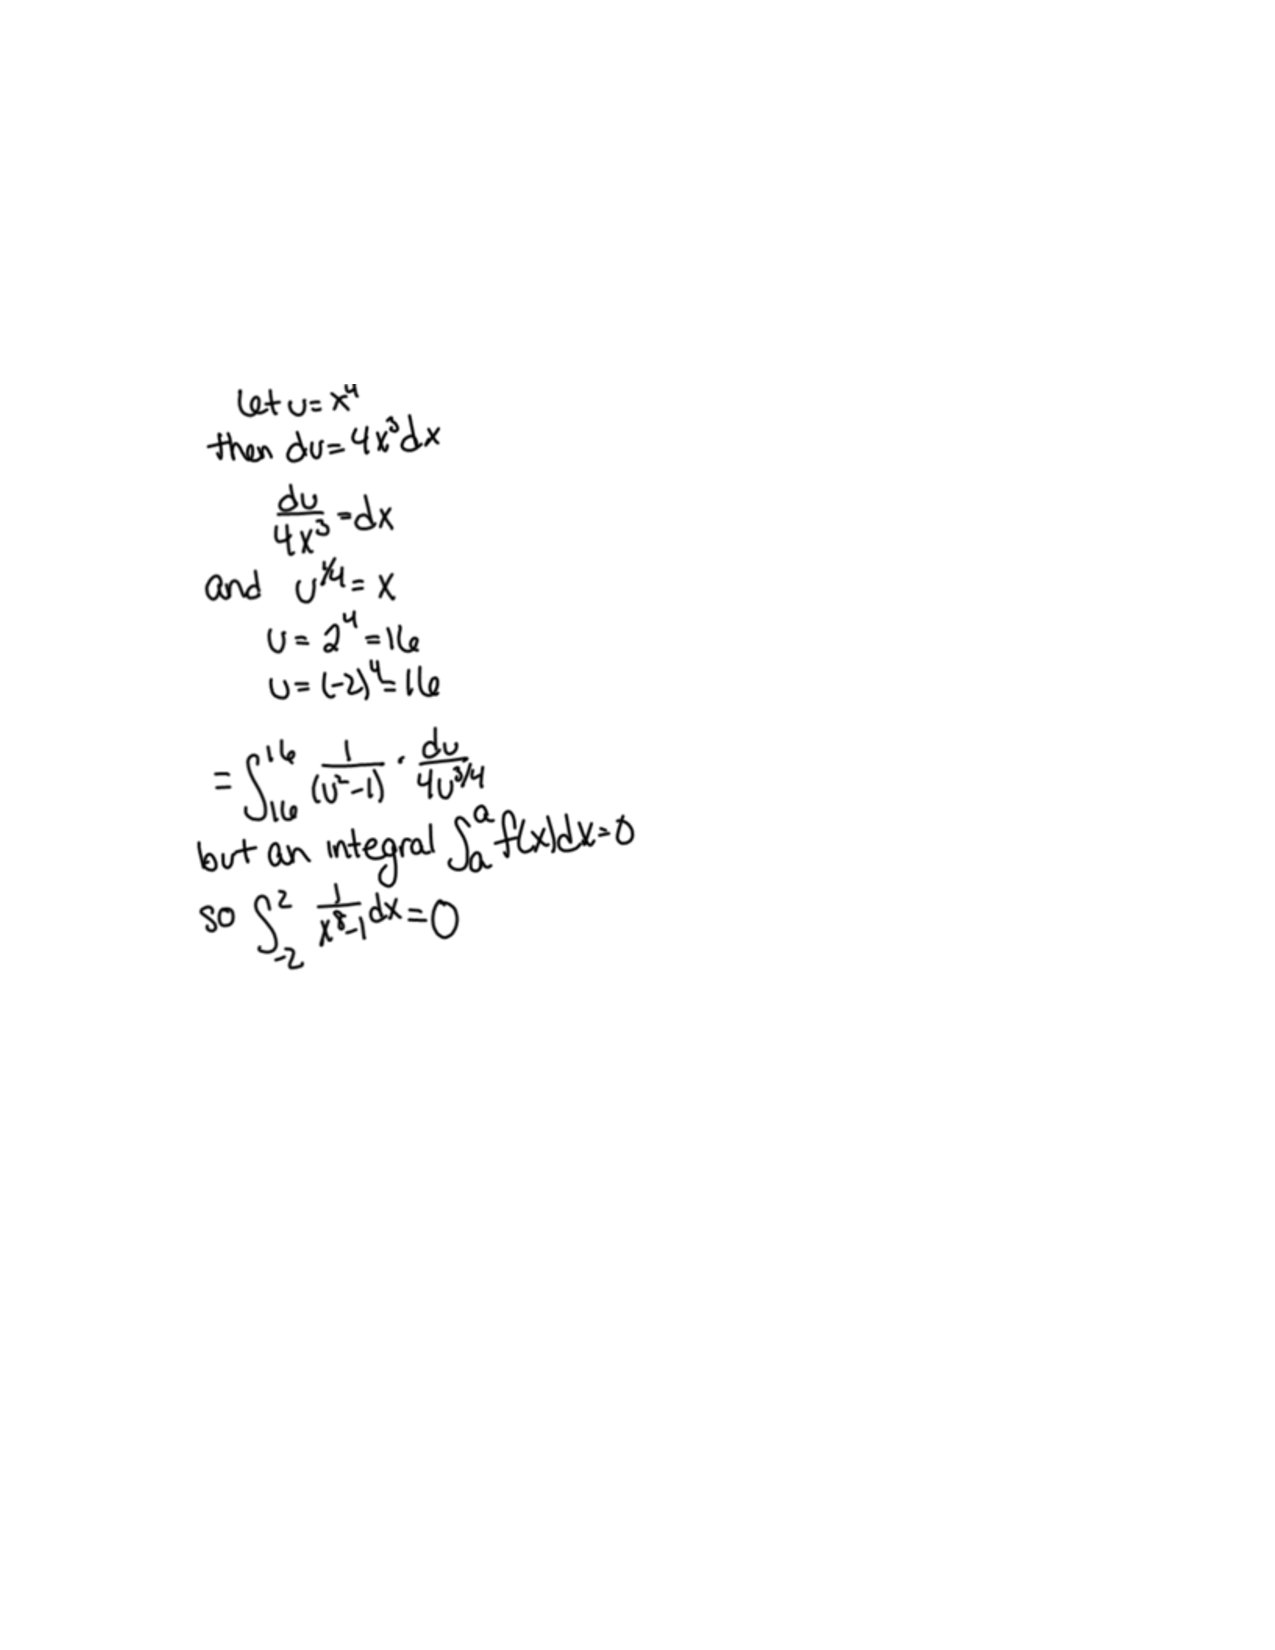
\includegraphics[trim= 170 420 250 180]{Figure1.pdf}
%\end{image}

%add a ``.'' below when used in a specific directory.
\newcommand{\RR}{\mathbb R}
\renewcommand{\d}{\,d}
\newcommand{\dd}[2][]{\frac{d #1}{d #2}}
\renewcommand{\l}{\ell}
\newcommand{\ddx}{\frac{d}{dx}}
\newcommand{\dfn}{\textbf}
\newcommand{\eval}[1]{\bigg[ #1 \bigg]}

\usepackage{multicol}

\renewenvironment{freeResponse}{
\ifhandout\setbox0\vbox\bgroup\else
\begin{trivlist}\item[\hskip \labelsep\bfseries Solution:\hspace{2ex}]
\fi}
{\ifhandout\egroup\else
\end{trivlist}
\fi} %% we can turn off input when making a master document

\title{Recitation \# 11: Partial fractions and Improper Integrals}  

\begin{document}
\begin{abstract}		\end{abstract}
\maketitle




\section{Warm up:}
True or False:  It is possible for a region to be infinitely long but have a finite area.
	\begin{freeResponse}
	True.  Consider the region below the curve $y=\frac{1}{x^2}$, $x \geq 1$.
	\end{freeResponse}
	
\begin{instructorNotes}

\end{instructorNotes}







\section{Group work:}



%problem 1
\begin{problem}
Without determining the coefficients, write the partial fraction decomposition of the following rational function:
	\[
	\frac{5x^{13} - 6x^{12} + 7x^3 - 5x - 18}{(2x-3)(5x+9)^3 (x^2+9x+19)(x^2+9x+21)^2}
	\]
	\begin{freeResponse}
	The degree of the numerator is $13$, whereas the degree of the denominator is $10$.  
	So if we perform long division, we will get a degree $13-10=3$ polynomial plus partial fractions for the remainder term:
		\begin{align*}
		&\frac{5x^{13} - 6x^{12} + 7x^3 - 5x - 18}{(2x-3)(5x+9)^3 (x^2+9x+19)(x^2+9x+21)^2} = Ax^3 + Bx^2 + Cx + D  \\
		&+ \frac{E}{2x-3} + \frac{F}{5x+9} + \frac{G}{(5x+9)^2} + \frac{H}{(5x+9)^3} + \frac{I}{x-i_1} + \frac{J}{x-i_2}  \\
		&+ \frac{Kx+L}{x^2+9x+21} + \frac{Mx+N}{(x^2+9x+21)^2}.
		\end{align*}
		
	\dfn{Explanation of $i_1$ and $i_2$:} 
	The quadratic $x^2+9x+19$ can be factored over the real numbers, since the discriminant $b^2-4ac = 81-76 > 0$.  
	The numbers $i_1$ and $i_2$ are the two real roots to this polynomial, ie
		\[
		i_1 = \frac{-9+\sqrt{5}}{2}	\qquad	i_2=\frac{-9 - \sqrt{5}}{2}.
		\]
	Note that the polynomial $x^2+9x+21$ is irreducible (over the real numbers) since its discriminant is less than $0$.  
	\end{freeResponse}
	
\end{problem}

\begin{instructorNotes}
Make sure that the students do not attempt to perform the long division.  
We are only looking for the \dfn{form} of the decomposition, which will be a cubic polynomial followed by a sum of rational functions.  
Note that $x^2 + 9x +19$ can be factored over the reals while $x^2 + 9x + 21$ cannot.  
This is a good time to talk about the descriminant.
\end{instructorNotes}







%problem 2
\begin{problem}
Evaluate:
	\[
	\int \frac{7x^3 + 18x + 9}{x^4 + 9x^2} \d x
	\]
{\it Hint:  If $f(x) = 7x^3 + 18x + 9$, then $f(2) = 101$, $f(1) = 34$, and $f(-1) = -16$.}
	\begin{freeResponse}
	First factor the denominator
		\[
		x^4 + 9x^2 = x^2(x^2 + 9).
		\]
	The we can decompose the integrand as a partial fraction
		\begin{equation*}
		\frac{7x^3+18x+9}{x^2(x^2+9)} = \frac{A}{x} + \frac{B}{x^2} + \frac{Cx+D}{x^2+9}
		\end{equation*}
		\begin{align*}
		\Longrightarrow	\quad	7x^3 + 18x + 9 &= Ax(x^2+9) + B(x^2+9) + (Cx+D)x^2  \\
		&= Ax^3 + 9Ax + Bx^2 + 9B + Cx^3 + Dx^2  \\
		&= (A+C)x^3 + (B+D)x^2 + 9Ax + 9B.
		\end{align*}
	By equating coefficients for powers of $x$ we have that
		\begin{align*}
		&9 = 9B 	\qquad	\Longrightarrow	\qquad	B = 1  \\
		&18=9A 	\qquad	\Longrightarrow	\qquad	A = 2  \\
		&0 = B+D 	\qquad	\Longrightarrow	\qquad	0 = 1 + D 	\qquad \Longrightarrow \qquad D = -1  \\
		&7=A+C 	\qquad	\Longrightarrow	\qquad	7=2+C 	\qquad \Longrightarrow \qquad C = 5.
		\end{align*}
	Thus
		\begin{align*}
		\int \frac{7x^3 + 18x + 9}{x^4 + 9x^2} \d x
		&= \int \left( \frac{2}{x} + \frac{1}{x^2} + \frac{5x-1}{x^2+9} \right) \d x  \\
		&= 2 \ln |x| - \frac{1}{x} + 5 \int \frac{x}{x^2 + 9} \d x - \int \frac{1}{x^2 + 9} \d x  \\
		&= 2 \ln |x| - \frac{1}{x} + \frac{5}{2} \ln (x^2 + 9) - \frac{1}{3} \arctan \left( \frac{x}{3} \right) + C.
		\end{align*}
	Note that, in the previous step, we substituted $u = x^2 + 9$ for the first integral and $u = \frac{x}{3}$ in the second integral.
	\end{freeResponse}
		
\end{problem}

\begin{instructorNotes}
First, note that students often have difficulty understanding that $x^2 = (x-0)^2$ is a perfect square of a linear factor $(x-0)$.  
The hint should help the students quickly solve for the unknowns.  
Using $x=0$ (not mentioned, but easily evaluated), one of the unknowns is immediately known.  
Using $1$ and $-1$ and adding the resulting equations finds a second unknown.  
Using $2$ will give them two equations and two unknowns to find the other two.  
The decomposition is
	\[
	\frac{2}{x} - \frac{1}{x^2} + \frac{5x-1}{x^2 + 9}.
	\]
\end{instructorNotes}












% Problem 4
\begin{problem}
Review of limits:
	\begin{enumerate}
	
	\item  $\lim_{x \to -\infty} \left( 3x^{-6} + e^{5x} + \frac{\sin x}{x^2 + 3} \right)$
	\begin{freeResponse}
	Recall that the limit of a sum is the sum of the limits, provided that those limits exist.
		\begin{itemize}
		\item  $\lim_{x \to -\infty} 3x^{-6} = \lim_{x \to -\infty} \frac{3}{x^6} = 0$.
		\item  $\lim_{x \to -\infty} e^{5x} = 0$.
		\item  $\lim_{x \to -\infty} \frac{\sin x}{x^2 + 3} = 0$  
		
		\vspace{8pt}
		
		{\color{red} \text{To rigorously prove this, you need to use the squeeze theorem.}}
		\end{itemize}
	Thus, 
		\[
		\lim_{x \to -\infty} \left( 3x^{-6} + e^{5x} + \frac{\sin x}{x^2 + 3} \right) = 0
		\]
	\end{freeResponse}
	
	
	
	\item  $\lim_{x \to \infty} \frac{x}{\sqrt{9x^2+4}}$
	\begin{freeResponse}
		\begin{align*}
		\lim_{x \to \infty} \frac{x}{\sqrt{9x^2+4}}
		&= \lim_{x \to \infty} \frac{x}{\sqrt{x^2} \cdot {\sqrt{9 + \frac{4}{x^2}}}}  \\
		&= \lim_{x \to \infty} \frac{x}{|x| \cdot \sqrt{9 + \frac{4}{x^2}}}  \\
		&= \lim_{x \to \infty} \frac{x}{x \cdot \sqrt{9 + \frac{4}{x^2}}}  \\
		&= \lim_{x \to \infty} \frac{1}{\sqrt{9 + \frac{4}{x^2}}}  \\
		&= \frac{1}{\sqrt{9 + 0}} = \frac{1}{3}.
		\end{align*}
	\end{freeResponse}
	
	
	
	\item  $\lim_{x \to -\infty} \arctan x$
	\begin{freeResponse}
	$\lim_{x \to -\infty} \arctan x = - \frac{\pi}{2}. $
	\end{freeResponse}
	
	\end{enumerate}
		
\end{problem}

\begin{instructorNotes}
Review of limits.
\end{instructorNotes}








%problem 5
\begin{problem}
In each of the following, determine if the given integral converges or diverges.  
If it converges, find the value.

	\begin{enumerate}
	
	\item  $\int_{-1}^{\infty} \frac{3}{2x+1} \d x$
	\begin{freeResponse}
	The function $\frac{3}{2x+1}$ has a vertical asymptote at $x=- \frac{1}{2}$.  
	So we rewrite the original integral as
		\[
		\int_{-1}^{\infty} \frac{3}{2x+1} \d x = \lim_{a \to -\frac{1}{2}^-} \int_{-1}^a \frac{3}{2x+1} \d x  
		+ \lim_{b \to -\frac{1}{2}^+} \int_b^0 \frac{3}{2x+1} \d x + \lim_{c \to \infty} \int_0^c \frac{3}{2x+1} \d x.
		\]
	The latter integral does not exist.  
	To see this, just note that
		\begin{align*}
		 \lim_{c \to \infty} \int_0^c \frac{3}{2x+1} \d x 
		 &= \lim_{c \to \infty} \eval{\frac{3}{2} \ln|2x+1|}_0^c  \\
		 &= \lim_{c \to \infty} \frac{3}{2} \ln|2c+1| = \infty.
		\end{align*}
	Therefore, 
		\[
		\int_{-1}^{\infty} \frac{3}{2x+1} \d x \; \text{ diverges.}
		\]
	\end{freeResponse}
	
	
	
	\item  $\int_{-\infty}^{\infty} x e^{-x} \d x$
	\begin{freeResponse}
	\[
	\int_{-\infty}^{\infty} x e^{-x} \d x = \lim_{a \to -\infty} \int_a^0 xe^{-x} \d x + \lim_{b \to \infty} \int_0^b xe^{-x} \d x.
	\]
	The first of these integrals does not exist.  
	To see this, we apply integration by parts
		\begin{align*}
		\lim_{a \to -\infty} \int_a^0 xe^{-x} \d x
		&= \lim_{a \to -\infty} \left( \eval{-xe^{-x}}_a^0 + \int_a^0 e^{-x} \d x \right)  \\
		&= \lim_{a \to -\infty} \left( \left[ 0 + ae^{-a} \right] + \eval{-e^{-x}}_a^0 \right)  \\
		&= \lim_{a \to -\infty} \left( ae^{-a} + e^{-a} - 1 \right)  \\
		&= \lim_{a \to -\infty} \left( e^{-a}(a+1) - 1 \right)  \\
		&= - \infty.
		\end{align*}
	Thus
		\[
		\int_{-\infty}^{\infty} x e^{-x} \d x \; \text{ diverges.}
		\]
	\end{freeResponse}
	
	
	
	\item  $\int_6^{\infty} \frac{2-4x}{2x^2 - 13x + 20} \d x$
	\begin{freeResponse}
	First notice that we can factor the denominator as
		\[
		2x^2 - 13x + 20 = (2x-5)(x-4).
		\]
	So we find a partial fraction decomposition of the integrand
		\begin{align*}
		&\frac{2-4x}{(2x-5)(x-4)} = \frac{A}{2x-5} + \frac{B}{x-4}  \\
		\Longrightarrow \qquad &2-4x = A(x-4) + B(2x-5).
		\end{align*}
	We can solve for $A$ and $B$ via the following substitutions:
		\begin{itemize}
		\item {\color{red}$\left( \text{Let } x=\frac{5}{2} \right)$} \quad $2 - 4 \left(\frac{5}{2} \right) = A \left(\frac{5}{2} - 4 \right)$  \\
			\[
			-8 = - \frac{3}{2} A \qquad \Longrightarrow \qquad A = \frac{16}{3}.
			\]
		\item {\color{red} (Let $x=4$)}  \quad $2-16 = 3B \qquad \Longrightarrow \qquad B = - \frac{14}{3}$.
		\end{itemize}
	Thus, 
		\begin{align*}
		\int_6^{\infty} \frac{2-4x}{2x^2 - 13x + 20} \d x
		&= \lim_{a \to \infty} \int_6^a \left[ \frac{\frac{16}{3}}{2x-5} - \frac{\frac{14}{3}}{x-4} \right] \d x  \\
		&= \lim_{a \to \infty} \eval{ \frac{8}{3} \ln|2x-5| - \frac{14}{3} \ln|x-4| }_6^a  \\
		&= \lim_{a \to \infty} \left[ \frac{8}{3} \left( \ln|2a-5| - \ln(7) \right) - \frac{14}{3} \left( \ln|a-4| - \ln(2) \right) \right]  \\
		&= \lim_{a \to \infty} \left[ \frac{1}{3} \left( \ln(2a-5)^8 - \ln(a-4)^{14} \right) - \frac{8}{3} \ln (7) + \frac{14}{3} \ln(2) \right]  \\
		&= \lim_{a \to \infty} \left[ \frac{1}{3} \ln \left( \frac{(2a-5)^8}{(a-4)^{14}} \right) - \frac{8}{3} \ln (7) + \frac{14}{3} \ln(2) \right]  \\
		&= - \infty.
		\end{align*}
	Thus,
		\[
		\int_6^{\infty} \frac{2-4x}{2x^2 - 13x + 20} \d x \; \text{ diverges.}
		\]
	\end{freeResponse}
	
	\end{enumerate}
	
\end{problem}

\begin{instructorNotes}
Make sure that students write in the limit notation throughout their work, with the limit taken after the definite integral has been evaluated.
	\begin{enumerate}
	\item has a vertical asymptote as well as a limit going to infinity.
	\item is by parts, and L'Hospital's Rule will be useful for the limit.
	\item will need partial fractions.  
	The coefficients of the decomposition are rigged to be opposites of each other, so that one can use properties of logarithms to aid in taking the limit.
	\end{enumerate}
\end{instructorNotes}







%problem 6
\begin{problem}
Find the volume of the solid whose base is the region where $x \geq 1$, $y \geq 0$, and below the curve $y=\frac{1}{x^4}$, and whose cross sections perpendicular to the $x$-axis are squares.
	\begin{freeResponse}
	The area of each cross-section is $\left( \frac{1}{x^4} \right)^2 = \frac{1}{x^8}$.  
	Thus,
		\begin{align*}
		{\color{red}\text{Volume }} &= \int_1^{\infty} \frac{1}{x^8} \d x  \\
		&= \lim_{a \to \infty} \eval{- \frac{1}{7 x^7}}_1^a  \\
		&= \lim_{a \to \infty} \left( - \frac{1}{7a^7} + \frac{1}{7} \right)  \\
		&= 0 + \frac{1}{7} = \frac{1}{7}.
		\end{align*}
	\end{freeResponse}

\end{problem}

\begin{instructorNotes}

\end{instructorNotes}










	
	
	
	
	
	
	
	
	

	










								
				
				
	














\end{document} 


















